\chapter{Arrays of Arrays}

The last two chapters of this book will use 2D graphics to illustrate advanced object-oriented concepts.
If you haven't yet read Appendix~\ref{graphics}, please do so now to become familiar with the \java{Canvas}, \java{Color}, and \java{Graphics} classes from the \java{java.awt} package.
We will use these classes to make graphical simulations.


\section{Conway's Game of Life}

A mathematician named John Conway invented the {\it Game of Life}, which he called a ``zero-player game'' because no players are needed to choose strategies or make decisions.
After you set up the initial conditions, you watch the game play itself.
That turns out to be more interesting than it sounds; you can read about it at \url{http://en.wikipedia.org/wiki/Conways_Game_of_Life}.

\begin{figure}[!ht]
\begin{center}
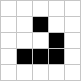
\includegraphics{figs/glider.png}
\caption{A ``Glider'' in the Game of Life.}
\label{fig:glider}
\end{center}
\end{figure}

The game consists of a two-dimensional grid of square cells.
Each cell is either ``alive'' or ``dead''; the color of the call indicates its status.
Figure~\ref{fig:glider} shows an example grid configuration.
The game proceeds in {\bf time steps}, during which every cell interacts with its {\bf neighbors} (adjacent cells).
At each step in time, the following rules are applied:

\begin{enumerate}
\item Any live cell with fewer than two live neighbors dies, as if by underpopulation.
\item Any live cell with more than three live neighbors dies, as if by overpopulation.
\item Any dead cell with exactly three live neighbors becomes a live cell, as if by reproduction.
\end{enumerate}

Notice some consequences of these rules.
If you start with a single live cell, it dies.
If all cells are dead, no cells come to life.
But if you have 4 cells in a square, they keep each other alive; that's a stable configuration.

Most simple starting configurations either die out quickly or reach a stable configuration.
But there are a few starting conditions that display remarkable complexity.
One of those is the R-pentomino: it starts with only five cells, runs for 1103 time steps, and ends in a stable configuration with 116 live cells (see
\url{http://www.conwaylife.com/wiki/R-pentomino}).

In the following sections, we will implement the Game of Life in Java.


\section{The Cell Class}

Using top-down design (see Section~\ref{shuffle}), it's clear that we'll need at least three classes: one for the cells, one for the grid, and one for the game itself.
We'll begin by designing the class for cells.

When drawing a cell, we'll need to know its coordinates on the screen.
We could use a \java{Rectangle} object (see Section~\ref{sec:Rectangle}) to store the cell's coordinates.
However, given that each cell is a square, we can represent its location with three integers: the \java{x} and \java{y} coordinates of the upper-left corner, and the \java{size} of the square (length of each side).
The cell will also need a \java{Color}.

Here is the beginning of the \java{Cell} class:

\begin{code}
public class Cell {
    private final int x;
    private final int y;
    private final int size;
    private Color color;
}
\end{code}

Notice that \java{x}, \java{y}, and \java{size} are constants.
Once the cell is created, we don't want it to move around accidentally.
Its \java{color}, on the other hand, is not a constant and might change frequently.

The next step is to write a constructor.
It's good practice to design classes to be reusable, and there are other games that might need to make cells.
We'll make a constructor that takes \java{x}, \java{y}, and \java{size} as parameters.

\begin{code}
public Cell(int x, int y, int size) {
    this.x = x;
    this.y = y;
    this.size = size;
    this.color = Color.WHITE;
}
\end{code}

In the following example, we use this constructor to create a \java{Cell}.
Its upper-left corner is at (0, 0), and the cell is 10x10 pixels wide.

\begin{code}
Cell cell = new Cell(0, 0, 10);
\end{code}

To draw a cell, we will take the graphics context as a parameter (similar to the \java{paint} method in Appendix~\ref{graphics}).
We then use \java{fillRect} to paint the cell itself and \java{drawRect} to paint a light gray border around it.

\begin{code}
public void draw(Graphics g) {
    g.setColor(this.color);
    g.fillRect(x + 1, y + 1, size - 1, size - 1);
    g.setColor(Color.LIGHT_GRAY);
    g.drawRect(x, y, size, size);
}
\end{code}

Finally, we will need methods for changing the cell's color.
We could just implement \java{getColor} and \java{setColor}.
But it will be more convenient if we design more specific methods.

For the Game of Life, the cells will either be dead (white) or alive (black).
To make the code reusable, we will refer to these states as ``off'' and ``on''.
And to improve readability, we will define class constants for these colors.
%So we will write boolean methods named \java{isOff} and \java{isOn} for getting the color, and void methods named \java{turnOff} and \java{turnOn} for setting the color.

\begin{code}
public static final Color OFF = Color.WHITE;
public static final Color ON = Color.BLACK;

public boolean isOff() {
    return color == OFF;
}
public boolean isOn() {
    return color == ON;
}
public void turnOff() {
    color = OFF;
}
public void turnOn() {
    color = ON;
}
\end{code}


\section{Two-Dimensional Arrays}

We can use an array to represent a grid of cells.
For example, we can represent a 5x5 grid with an array of 25 cells.
The following code is similar to how we created an array of cards in Section~\ref{cardarray}:

\begin{code}
Cell[] array = new Cell[25];
for (int r = 0; r < rows; r++) {
    int y = r * SIZE;
    for (int c = 0; c < cols; c++) {
        int x = c * SIZE;
        array[r * 5 + c] = new Cell(x, y, SIZE);
    }
}
\end{code}

The loop variables \java{r} and \java{c} are the row and column indexes of each cell, and the variables \java{x} and \java{y} are the coordinates of each cell.
For example, if \java{SIZE} is 10 pixels, then the cell at index (2, 2) would be at coordinates (20, 20).

The expression \java{array[r * 5 + c]} calculates the index of the row and column in the array.
For example, the array index of the cell at (1, 2) would be 7.
Figure~\ref{fig:1D-array} illustrates how the rows are arranged.

\begin{figure}[!ht]
\begin{center}
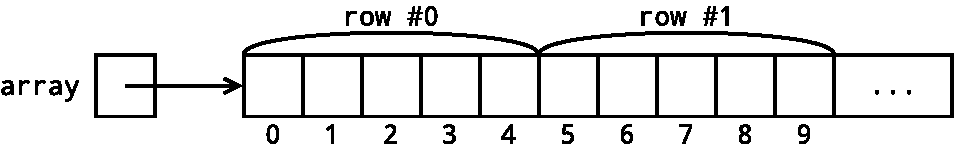
\includegraphics[width=366pt]{figs/1D-array.pdf}
\caption{Storing rows and columns with an array.}
\label{fig:1D-array}
\end{center}
\end{figure}

This way of represdenting two-dimensional data is know as {\bf row-major order}, because the objects are stored row by row.
A more natural way to represent multidimensional data is to use multidimensional arrays, or arrays of arrays, as shown in Figure~\ref{fig:2D-array}.

\begin{figure}[!ht]
\begin{center}
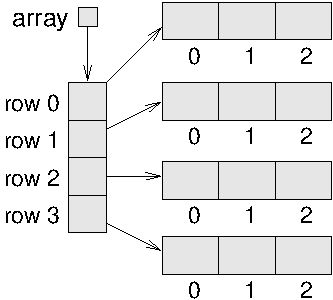
\includegraphics[width=265pt]{figs/2D-array.pdf}
\caption{Storing rows and columns with an array of arrays.}
\label{fig:2D-array}
\end{center}
\end{figure}

Using arrays of arrays makes it easier to refer to individual cells by row and column indexes.
We can rewrite the previous code by making two changes:

\begin{center}
\begin{tabular}{rl}
Replace: & \java{Cell[] array = new Cell[25];} \\[-1ex]
   With: & \java{Cell[][] array = new Cell[5][5];} \\[1ex]
Replace: & \java{array[r * 5 + c] = new Cell(x, y, SIZE);} \\[-1ex]
   With: & \java{array[r][c] = new Cell(x, y, SIZE);} \\
\end{tabular}
\end{center}

Notice that we no longer need to calculate \java{array[r * 5 + c]}.
The expression \java{array[r]} gets the array at index \java{r}, after which \java{[c]} gets the cell at index \java{c}.


\section{The GridCanvas Class}

Now that we have a \java{Cell} class and a way of representing a two-dimensional array of cells, we can design a class to represent a grid of cells.
We will encapsulate the code from the previous section and generalize it to construct a grid of any size:

\begin{code}
public class GridCanvas extends Canvas {
    private Cell[][] array;

    public GridCanvas(int rows, int cols, int size) {
        array = new Cell[rows][cols];
        for (int r = 0; r < rows; r++) {
            int y = r * size;
            for (int c = 0; c < cols; c++) {
                int x = c * size;
                array[r][c] = new Cell(x, y, size);
            }
        }

        // set the canvas size
        setSize(cols * size, rows * size);
    }
}
\end{code}

\index{IS-A}
\index{HAS-A}

Using the terminology from the previous chapter, \java{GridCanvas} ``IS-A'' \java{Canvas} that ``HAS-A'' two-dimensional array of cells.
By extending the \java{Canvas} class from \java{java.awt}, we inherit methods for drawing cells on the screen.

In fact, that code is surprisingly straightforward.
To draw the grid, we simply draw each cell.
We use nested \java{for} loops to traverse the array of arrays:

\begin{code}
public void draw(Graphics g) {
    for (Cell[] row : array) {
        for (Cell cell : row) {
            cell.draw(g);
        }
    }
}
\end{code}

It's helpful to read the previous code in English: ``For each \java{row} in the grid \java{array}, and for each \java{cell} in the \java{row}, draw the \java{cell} in the graphics context.''
Each cell knows how to draw itself, because the coordinates are built-in.

The \java{Canvas} class provides two methods, \java{paint} and \java{update}, that are called to draw its contents.
These methods are intended to be overridden by the subclass to perform the actual painting and updating.
We will simply make them call the \java{draw} method, which paints (or updates) the entire Canvas.

%The default behavior of \java{paint} is simply to clear the \java{Canvas}; it's expected that a subclass will override this method.
%The default behavior of \java{update} is to clear the \java{Canvas} and then call \java{paint}.

\begin{code}
public void paint(Graphics g) {
    draw(g);
}
public void update(Graphics g) {
    draw(g);
}
\end{code}

In additional to drawing, we will provide methods for working with the grid itself.
It will be useful to know how many rows and columns the grid has.
This information is built into the array of arrays:

\begin{code}
public int numRows() {
    return array.length;
}
public int numCols() {
    return array[0].length;
}
\end{code}

Recall that \java{array} (the variable) is an array of rows.
So the number of rows is equal to the length of \java{array}.
Since the grid is rectangular, each row has the same number of columns.
So the number of columns is the length of \java{array[0]}, or any other index for that matter.

Finally, we will write methods for working with individual cells.
The first method returns the \java{Cell} at (\java{r}, \java{c}), and the second method turns a \java{Cell} on.

\begin{code}
public Cell cellAt(int r, int c) {
    return array[r][c];
}
public void init(int r, int c) {
    array[r][c].turnOn();
}
\end{code}